\section{MARF Architecture}
\noindent
\rule{7.0in}{.013in}

Before we begin, you should understand the basic
MARF  system  architecture. Understanding how the
parts of MARF interact will make the next sections
somewhat clearer. This document presents architecture
of the MARF system, including the layout of the physical
directory structure, and Java packages.

Let's take a look at the general MARF structure in Figure \ref{fig:arch}.
The MARF class is the central ``server'' and configuration placeholder which major method -
the core pipeline - a typical pattern recognition process.
The figure presents basic abstract modules of the architecture.
When a developer needs to add or use a module, they derive
from the generic ones,

\begin{figure}
	\centering
	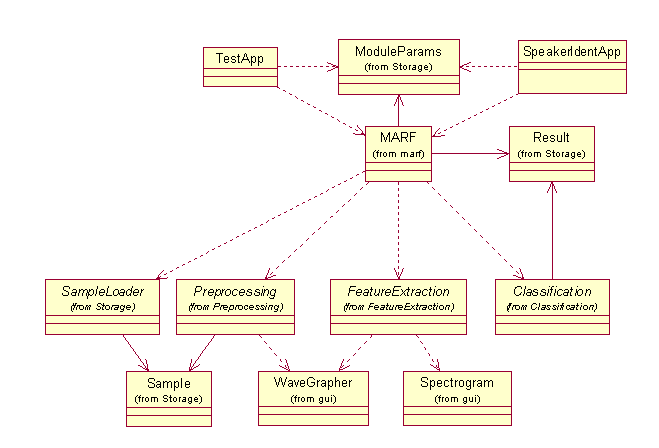
\includegraphics[angle=90]{../graphics/arch/arch-general.png}
	\caption{Overall Architecture}
	\label{fig:arch}
\end{figure}

The core pipeline sequence diagram from an application
up until the very end result is presented on Figure \ref{fig:pipeline}. It includes all major
participants as well as basic operations. The participants are the
modules responsible for a typical general pattern recognition pipeline.

\begin{figure}
	\centering
	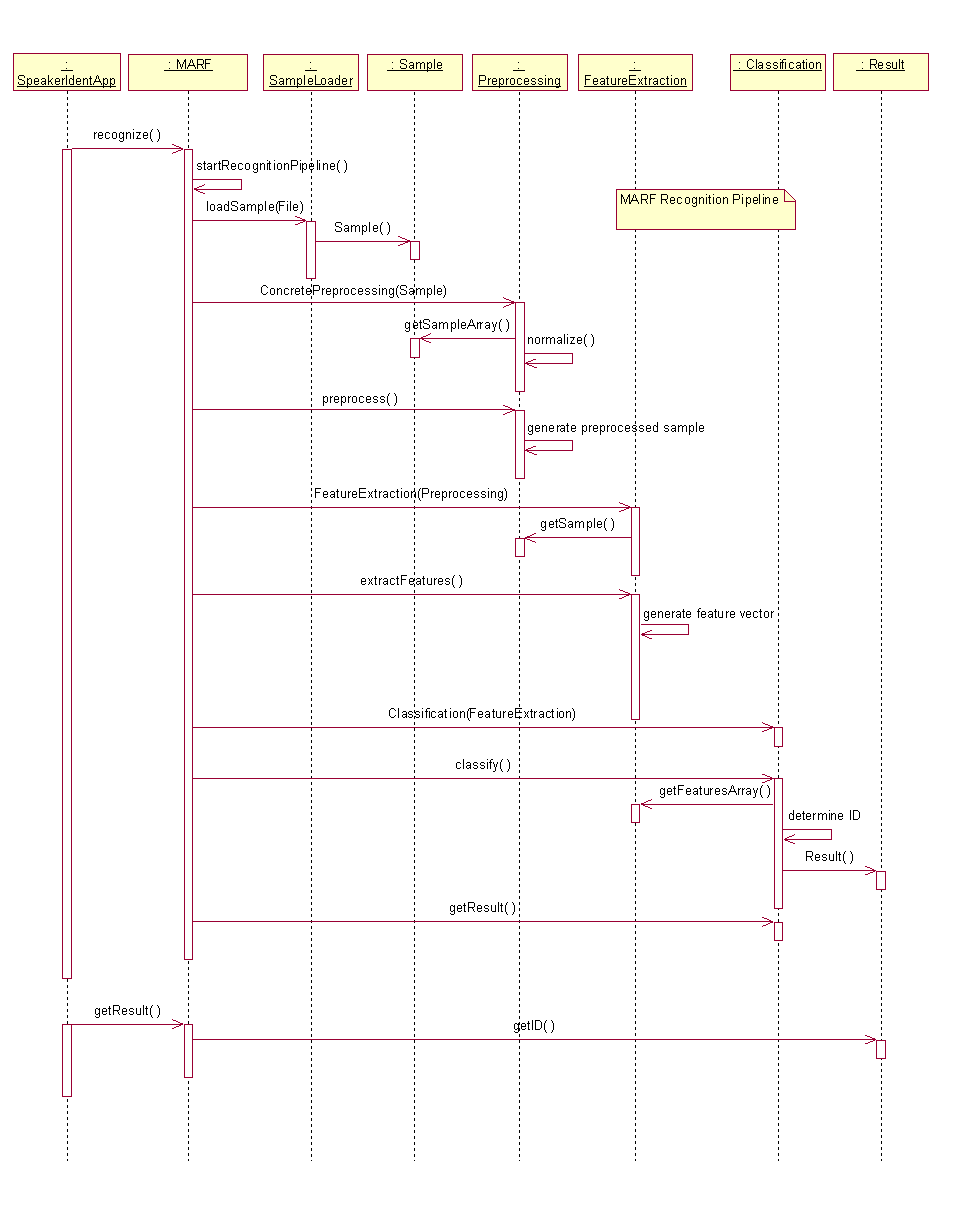
\includegraphics[angle=90,totalheight=660pt,width=550pt]{../graphics/arch/pipeline.png}
	\caption{The Core Pipeline}
	\label{fig:pipeline}
\end{figure}

Consequently, the framework has the mentioned basic modules,
as well as some additional entities to manage storage
and serialization of the input/output data.

\subsection{Application Point of View}

An application, using the framework, has to choose
the concrete configuration and submodules for preprocessing,
feature extraction, and classification stages. There is an API the application
may use defined by each module or it can use them through the MARF.

There are two phases in MARF's usage by an application:

\begin{itemize}
	\item Training, i.e. \verb+train()+
	\item Recognition, i.e. \verb+recognize()+
\end{itemize}

Training is performed on a virgin MARF installation to get
some training data in. Recognition is an actual identification process of a sample
against previously stored patterns during training.

\subsection{Packages and Physical Layout}

\begin{figure}
	\centering
	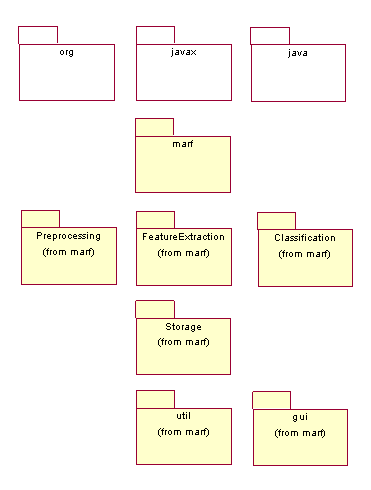
\includegraphics{../graphics/arch/packages.png}
	\caption{MARF Java Packages}
	\label{fig:packages}
\end{figure}

The Java package structure is in Figure \ref{fig:packages}.
The following is the basic structure of MARF:

\vspace{15pt}
\hrule
\begin{verbatim}
marf.*

MARF.java - The MARF Server
            Supports Training and Recognition mode
            and keeps all the configuration settings.

marf.Preprocessing.* - The Preprocessing Package

/marf/Preprocessing/

   Preprocessing.java - Abstract Preprocessing Module, has to be subclassed

   /Endpoint/*.java   - Endpoint Filter as implementation of Preprocessing
   /Dummy/*.java
   /FFTFilter/
       FFTFilter.java
       LowPassFilter.java
       HighPassFilter.java
       BandpassFilter.java - Bandpass Filter as implementation of Preprocessing
       HighFrequencyBoost.java

marf.FeatureExtraction.* - The Feature Extraction Package

/marf/FeatureExtraction/
    FeatureExtraction.java
    /FFT/FFT.java        - FFT implementation of Preprocessing
    /LPC/LPC.java        - LPC implementation of Preprocessing
    /Cepstral/*.java
    /Segmentation/*.java
    /F0/*.java

marf.Classification.* - The Classification Package

/marf/Classification/
    Classification.java
    /NeuralNetwork/NeuralNetwork.java
    /Stochastic/*.java
    /Markov/*.java
    /Distance/
       Distance.java
       EuclideanDistance.java
       ChebyshevDistance.java
       MinkowskiDistance.java
       MahalonobisDistance.java

marf.Storage.* - The Physical Storage Management Interface

/marf/Storage/
    Sample.java
    ModuleParams.java
    TrainingSet.java
    Result.java
    StorageManager.java - Interface to be implemented by the above modules
    SampleLoader.java   - Should know how to load different sample format
    /Loaders/*.*        - WAV, MP3, ULAW, etc.

marf.Stats.* - The Statistics Package meant to collect various types of stats.

/marf/Stats/
    StatsCollector.java - Time took, noise removed, patterns stored, modules available, etc.

marf.gui.* - GUI to the graphs and configuration

/marf/gui/
    Spectrogram.java
    WaveGrapher.java
\end{verbatim}
\hrule
\vspace{15pt}

\subsection{Current Limitations}

Our current pipeline is maybe somewhat too
rigid.  That is, there's no way to specify more than one preprocessing
or feature extraction module to process the same sample in one pass.
(In the case of preprocessing one filter may be used
along with normalization together, or just normalization by itself).

Also, it assumes that the whole sample is loaded before doing
anything with it, instead of sending parts of the sample a bit at a time.
Perhaps this simplifies things, but it won't allow us to deal with large
samples at the moment. However, it's not a problem for our framework
and the application since memory is cheap and samples are not too big. Additionally,
we have streaming support already in the \verb+WAVLoader+ and some modules support it, but
the final conversion to streaming did not happen in this release.

MARF provides only limited support for inter-module dependency. It is possible
to pass module-specific arguments, but problems like
number of parameters mismatch between feature extraction and classification,
and so on are not tracked.
